\documentclass{egpubl}
\usepackage{eg2017}

\Poster      % uncomment for (final) Short Conference Presentation

\electronicVersion % can be used both for the printed and electronic version

\ifpdf \usepackage[pdftex]{graphicx} \pdfcompresslevel=9
\else \usepackage[dvips]{graphicx} \fi

\PrintedOrElectronic

% prepare for electronic version of your document
\usepackage{t1enc,dfadobe}

\usepackage{egweblnk}
\usepackage{cite}

%%% Added packages and commands %%%
\usepackage[usenames,dvipsnames]{xcolor}
\usepackage{amsmath}
\usepackage{amssymb}
\usepackage{hyperref}

\newcommand{\added}[1]{{\color{Red}\textbf{#1}}} % do not need this probably
\newcommand{\note}[3]{{\color{#2}\textbf{#1: #3}}}
\newcommand{\henrik}[1]{\note{HENRIK}{WildStrawberry}{#1}}
\newcommand{\john}[1]{\note{JohnKa}{RubineRed}{#1}}
\newcommand{\unsure}[1]{\note{USIKKER}{Green}{#1}}
\newcommand{\IGNORE}[1]{}
\graphicspath{{fig/}}

% correct bad hyphenation here
\hyphenation{to-po-lo-gi-cal-ly to-po-lo-gy      ini-tial  col-our pat-ches}

\title[Non-rectangular gradient mesh tool]
{A Gradient Mesh Tool for Non-Rectangular Gradients}

% for anonymous conference submission please enter your SUBMISSION ID
% instead of the author's name (and leave the affiliation blank) !!
\author[short1007]
{\parbox{\textwidth}{\centering short1007}
	\\
	% School/Institution here (if accepted)
	{\parbox{\textwidth}{\centering } }
}

% if the Editors-in-Chief have given you the data, you may uncomment
% the following five lines and insert it here
%
% \volume{27}   % the volume in which the issue will be published;
% \issue{1}     % the issue number of the publication
% \pStartPage{1}      % set starting page

\begin{document}
	
	% \teaser{
	%  \includegraphics[width=\linewidth]{eg_new}
	%  \centering
	%   \caption{New EG Logo}
	% \label{fig:teaser}
	% }
	
	\maketitle
	
	\begin{abstract}
		The gradient mesh tool, implemented in vector graphics software like Adobe Illustrator, is a much-used tool for creating and manipulating complex colour gradients. The mesh-based tool is restricted to rectangular control meshes, making it hard for the user to work with more complicated shapes such as shapes with holes. We propose a new gradient mesh tool that supports non-rectangular control meshes, with native support for a wide range of different shapes. Additionally, our tool supports flexible mesh and \colorbox{yellow}{colour editing} functionality that makes local edits easier than with previous tools. A user study indicates that our tool is easier to use in the setting of drawing colour gradients inside complicated shapes with holes.
		
		\begin{classification} % according to http:http://www.acm.org/about/class/1998
			\CCScat{Computer Graphics}{I.3.4}{Graphics Utilities}{Paint systems}
		\end{classification}
		
	\end{abstract}
	
	\section{Introduction}
	\label{sec:intro}
	
	In vector graphics design, working with complex colour functions is challenging. The restrictions of the linear gradient tool is one reason designers turn to pixel-based tools, like Adobe Photoshop, when the design turns complicated. This issue has been acknowledged in the research community and a wide range of different approaches have been proposed to make the design of colour gradients more effortless \cite{Orzan:2008,Lopez-Moreno:2013, Vergne:2012, Shao:2012}.
	
	The gradient mesh tool found in current vector graphics packages is a much-used tool for complex colour gradient design.	It is useful in scenarios where the linear gradient tool does not suffice. However, it does not support non-rectangular gradients: the control mesh which the user interacts with must be of rectangular topology. In this paper, we propose a new tool for gradient mesh editing where the user can create and manipulate non-rectangular colour gradients, like the one shown in Fig.[REF-teaser]. Our approach takes advantage of a recent gradient mesh interpolation technique that supports arbitrary mesh topology~\cite{Lieng:2016}. Being able to model non-rectangular gradient meshes provides significant practical advantages, especially for vector shapes with holes.
	
	\begin{figure}
		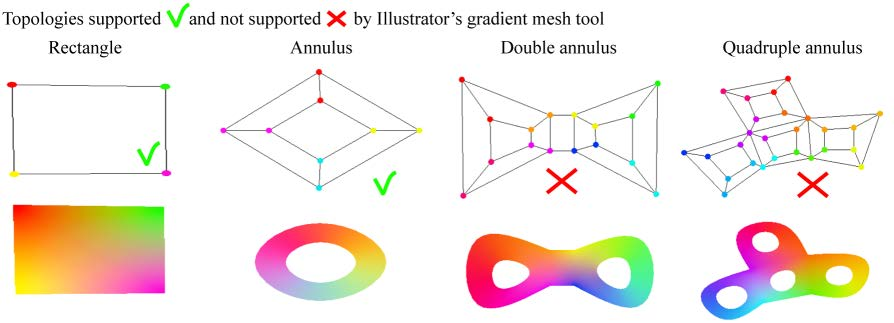
\includegraphics[]{illustratorVsOur.jpg}
		\caption{Caption... Image courtesy of Lieng et al. \cite{Lieng:2016}}
		\john{Should we use a new image, or is it OK to refer to the article and alter some of the original caption?}
		\label{fig:IllustratorVsOur}
	\end{figure}
	
	\section{Problem description}
	\label{sec:overview}
	
	In previous gradient mesh tools, with reference to Adobe Illustrators too, there are two approaches to mesh creation. The first option converts a vector graphics object compatible with rectangular gradient (i.e. a vector shape without holes) to a grid of control points. The user is required to input the number of rows and columns of the to-be gradient mesh. The creation is dependent on a grid representation, and is therefore incompatible with non-rectangular gradient meshes.
	
	The second option is a point-and-click interface where the user clicks on a location inside the target shape and a new control point is created at the clicked location. This is attractive as the creation operation is independent from the underlying data structure and can give rise to several interpretations. However, the interaction produces a global alteration: when a control point is added, a new row and column is added to the entire mesh. It is therefore challenging to achieve local gradient edits and the user must consequently plan the structure of the mesh so that the number of rows and columns is kept to a minimum. For an non-rectangular setting, this would be even more challenging. Fig.~\ref{fig:adHocPentagon} illustrates a point-and-click interaction inside a polygon adjacent to a pentagon. The effect of such an interaction is ambiguous and the solution will be ad-hoc.
	
	In conclusion, the user interaction already supported by the gradient mesh tool is hard to extend to the more flexible setting of non-rectangular control meshes.
	
	\begin{figure}[t]
		\centering
		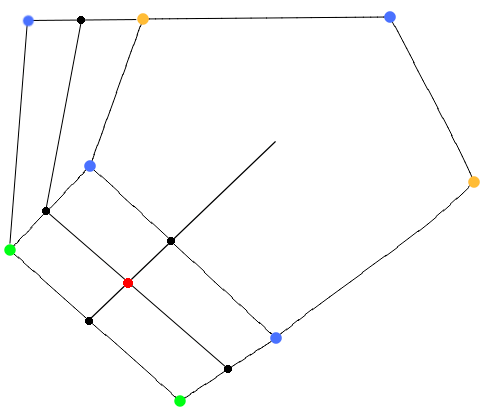
\includegraphics[height=0.25\textheight]{pentagonMesh.png}
		\caption{The red point indicates the location of were the user clicked. A new control point is made at this location. As mentioned in Section~\ref{sec:overview}, a new column and row is added to the entire mesh. New vertices are introduced at each edge intersection (represented as black points). The challenge occurs when we add a new vertex in a polygon adjacent to a pentagon. If the pentagon are split following the red dashed line we will suddenly introduce several new vertices as the line will propagate to adjacent polygons or introduce a T-junction if the line does not propagate. The solution will indeed be ad-hoc either way, and produce a mesh that is of poorer quality compared to the original mesh.
		}
		\john{TODO: Kutte ned paa tekst}
		\label{fig:adHocPentagon}
	\end{figure}
	
	\section{Tools for creating non-rectangular gradient meshes}
	\label{sec:method}
	
	Our approach takes inspiration from the pen tool found in SketchUp (\url{http://www.sketchup.com/}). Building on such a basic tool for creating polygonal meshes in 2D, we provide tools for operations such as face deletion, and edge split and collapse.
	
	The user to create initial meshes \textit{face-by-face}, which can later be refined and manipulated. Our \textbf{line tool} enables the user to create a single polygonal face. The user starts by creating a single face. The mesh is then expanded by iteratively adding faces to it. To add a face, the user selects an existing mesh vertex and place new control points on the canvas. The face is closed by clicking on an existing vertex that is connected to a face. If the initial vertex closes the face a non-manifold mesh can be achieved as shown in Fig.~\ref{fig:nonManifoldHoleMesh}.
	
	The user can further locally edit and refine the control mesh. The \textbf{edge split tool} splits a selected edge into two pieces. The inserted control point should then be connected to another mesh point to avoid valence-2 control points. Note that edges are modelled as cubic Bezier curves: each control point is associated with a gradient constraint for each of its edges that control the local influence of the colour of the control point. Such gradient constraints is a standard feature of gradient meshes. To ensure that the curve of the edge is maintained when the edge is split, the position of the new control point is calculated using De Casteljau's algorithm. Finally, adjacent edges can be collapsed for mesh simplification, and faces can be removed to introduce holes (Fig. REF).
	
	\begin{figure}[t]
		\centering
		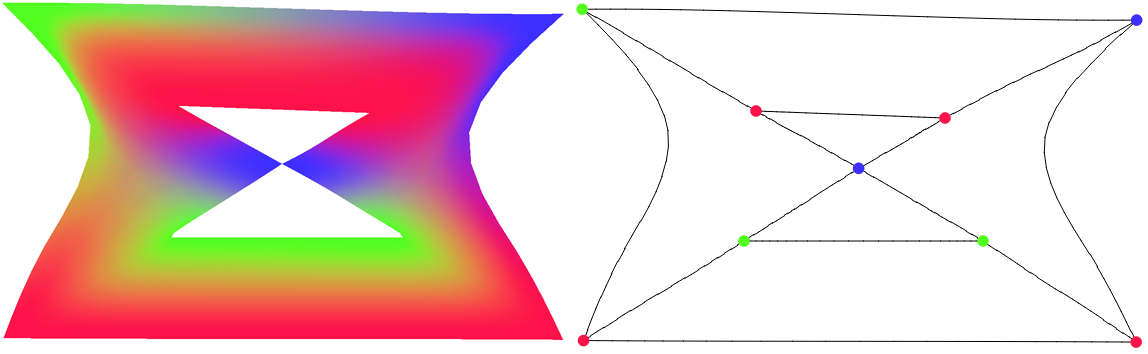
\includegraphics[height=0.25\textheight]{HoleAndNonManifoldMesh.png}
		\caption{Top: A non-manifold mesh with internal holes. Bottom: The control mesh.}
		\label{fig:nonManifoldHoleMesh}
	\end{figure}
	
	\section{Results and informal user study}
	\label{sec:results}
	
	TODO: results, Half-edge datastructure. Rewrite informal user study
	
	Our gradient mesh tool were tested by 5 subjects -- 2 professionals designers and 3 art students --- who all had experience with Adobe Illustrator. The subjects were given an introduction to our program and to the relevant tools in Illustrator. They were given two task; the first task was to make a rectangular gradient mesh. The second task was to make a gradient mesh with two holes. The subjects were not allowed to use layering, that is, none of the meshes should overlap. The tests were complemented with an user survey, which 4 of 5 test subjects answered.
	
	One test subject answered the following in the user survey: \textit{"[...] I enjoyed the experience from the tested tool more than Illustrator when it came to the tasks given. Both were difficult for a beginner, but at least the tested tool made more sense: especially with deleting frames to create holes."}.
	
	\section{Future work}
	\label{sec:FW}
	
	Though our gradient mesh tool offers opportunities to work with non-rectangular gradient meshes, it is not an full experience graphical design software application. Future work will be to rewrite our tool as a plug-in for the Adobe Illustrator. This presents several issues, as the underlying mesh representation in Illustrator differs from ours. One approach can be to take use of Pixar's OpenSubdiv library (\url{http://graphics.pixar.com/opensubdiv/}) to integrating our solution with Illustrators SDK.
	
	\section{Conclusion}
	
	We have introduced a new tool for working with non-rectangular gradient meshes. In contrast to gradient mesh tools in other applications -- like Adobe Illustrator -- our tool allows for quick and easy creation and alternation of gradient meshes which can be of arbitrary topology and contain holes. \unsure{Users are given more detailed control over the resulting mesh than with previous tools, as they easily can employ use of colour points and multi resolution editing of the mesh.}  \john{Har ikke nevnt noe om colour points eller multi res tidligere, saa kanskje ha noe annet her/fjerne det... Burde kanskje skrive mer her}
	
	\bibliographystyle{eg-alpha}
	
	\bibliography{refs}
	
\end{document}